\subsection{Detection}

By training the two classifiers (SVM and Logistic Regression) we obtain very similar results. In both cases the training accuracy is very close to, or even $100\%$. We do multiple runs since the data used to train $\mathcal{C}$ is drawn at random. This suggests that the decision boundary is very far from the regions of interest for the two classes, meaning that the LID is a good measure for detecting adversarial attacks. We next considering a test set, composed of about 2,000 images for each of the adversarial and non-adversarial attacks. We obtain no false positives on either of the classifiers, and a single false negative. This is shown in Figure .
\begin{figure}[!h]
\centering
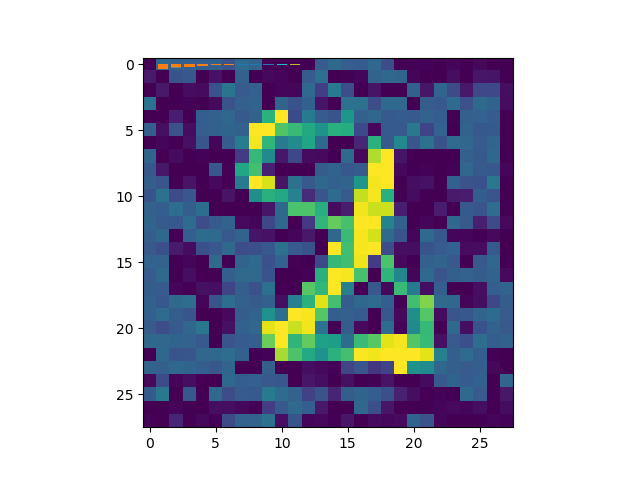
\includegraphics[scale=0.8]{eightthree.png}
\caption{Perturbed image of 8, misclassified as a 3.}
\end{figure}
We note that we have also tried training the classifiers directly on the PCA reduced features for each layer, $\mathbf{x} =(\boldsymbol{\phi}_1,\boldsymbol{\phi}_2,\boldsymbol{\phi}_3,\boldsymbol{\phi}_4)$, but we obtain performance that is only slightly better than random, for both the training and the test stages. This means that this feature vector is not appropriate for capturing whether the data is adversarial or not. This also confirms that LID is an appropriate measure for this.